\section{Exercise 2 - Design patterns }
\subsection{Exercise 2.1 - Singleton}
Before this sprint iteration, the project already contained an implementation of the singleton design pattern. The implementation of the singleton pattern is in the logger class. The singleton pattern ensures a class has only one instance. The singleton pattern also gives a global point to access this instance. The advantage of using a singleton pattern, is that you ensure that not two of the same objects are created. This could be important for object that only could have one instance. This is for example as used in this project the logger class, but could also be another class from which only one instance should be created.  The singleton pattern is implemented by making the constructor of this class private and creating a seperate getInstance mathod. This way you can ensure there is always one unique object of this class. The getInstance method and the logger instance variable are static, because they are used in a static way. Problems that could occur with this pattern is that you still can create two instances with singleton. This can happen when you use conccurent programming. By adding the volatile keyword it is ensured that threads handle the unique instance variable correctly when it is being initialized to the singleton instance.
Another way to prevent this problem is by adding the synchronized keyword to the getInstance method. This forces every thread to wait its turn before it can enter the method.

\subsection{Exercise 2.2 - Singleton}
Figure \ref{fig:2-2singleton} contains the UML Class diagram for the singleton design pattern concerning the logger.

\begin{figure}[ht!]
\centering
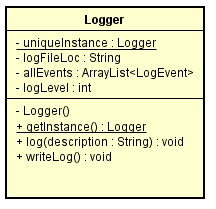
\includegraphics[width=5cm]{logger.jpg}
\caption{Singleton UML Class Diagram}
\label{fig:2-2singleton}
\end{figure}
\newpage

\subsection{Exercise 2.3 - Singleton}
Figure \ref{fig:2-3singleton} contains the UML Sequence diagram for the singleton design pattern in the logger. It contains two calls of the getInstance method from two example classes. In the first call the unique instance of the logger is created. In the second call the instance already exists so this is simple returned. 

\begin{figure}[ht!]
\centering
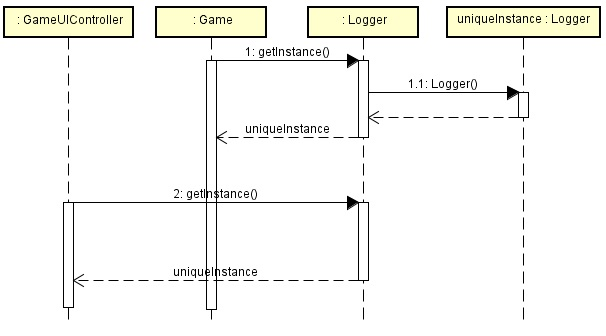
\includegraphics[width=13cm]{loggerSequence.jpg}
\caption{Singleton UML Sequence Diagram}
\label{fig:2-3singleton}
\end{figure}

\subsection{Exercise 2.1 - Observer}
In this sprint sound effects were created, for this new feature the observer pattern is used. The observer pattern ensures, when an observable object is changed the observer is notified. In the implementation for the sound effects is the soundcontroller the observer and the objects that could generate a sound by change the observables. This are for example the explosion objects which should generate an explosion sound. To implement this roles as observer and observable the interfaces observable and observer are implemented. An advantage of using the observer pattern instead of adding a method call to the soundcontroller in the  the explosion class is that this way objects are loosely coupled. The objects can interact with each other but have very little knowledge of each other. It is also easy to add new observers withoud changing the observable class. 

\newpage

\subsection{Exercise 2.2 - Observer}
Figure \ref{fig:1-2sounds} contains the UML Class diagram for the observer design pattern concerning the sound effects.

\subsection{Exercise 2.3 - Observer}
Figure .... contains the UML sequence diagram for the observer design pattern concerning the sound effects.